\begin{figure}[!ht]
    \centering
    \setlength{\resLen}{1.4in}
    \addtolength{\tabcolsep}{-3.5pt}
    \begin{tabular}{cc|cc}
        \multicolumn{2}{c|}{\textbf{(a)} Negatively correlated particles} &
        \multicolumn{2}{c}{\textbf{(b)} Positively correlated particles}
        \\
        \multicolumn{2}{c|}{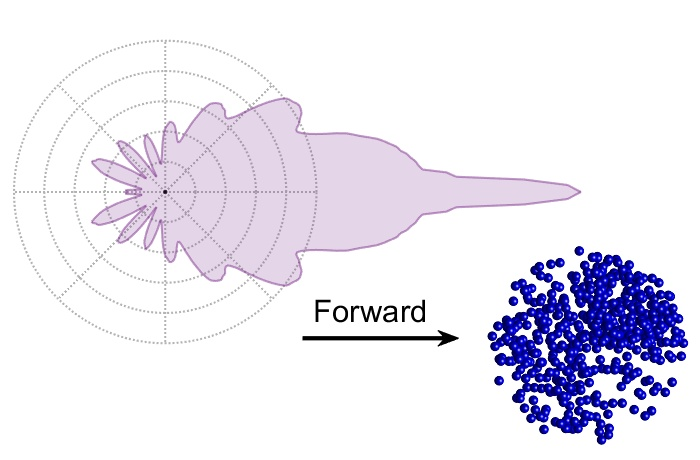
\includegraphics[width=2\resLen]{waveoptics/pfunc/neg_merge.jpg}} & \multicolumn{2}{c}{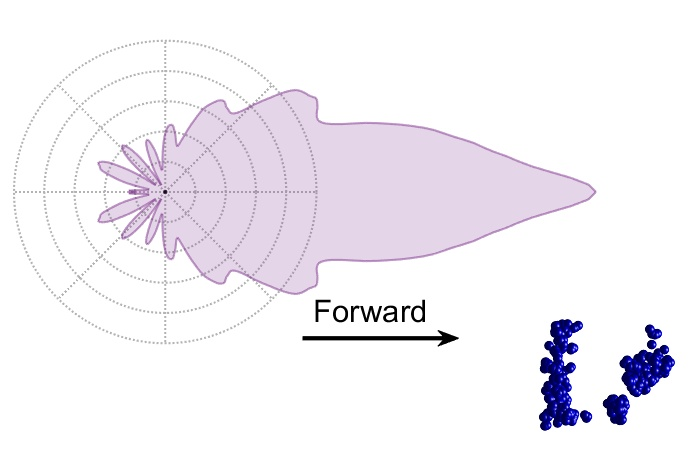
\includegraphics[width=2\resLen]{waveoptics/pfunc/pos_merge.jpg}} 
        \\
        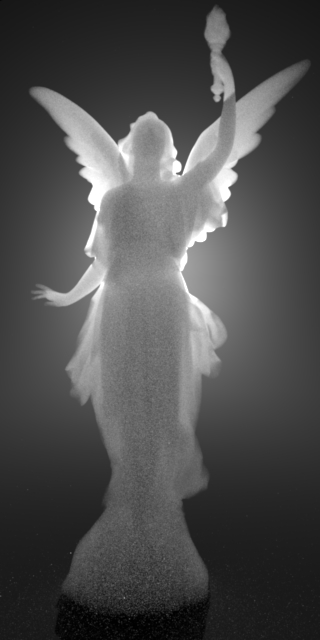
\includegraphics[width=\resLen]{waveoptics/lucy/neg_unc.jpg} &
        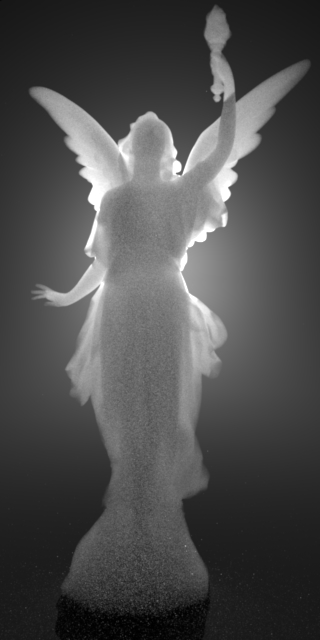
\includegraphics[width=\resLen]{waveoptics/lucy/neg_neg.jpg} &
        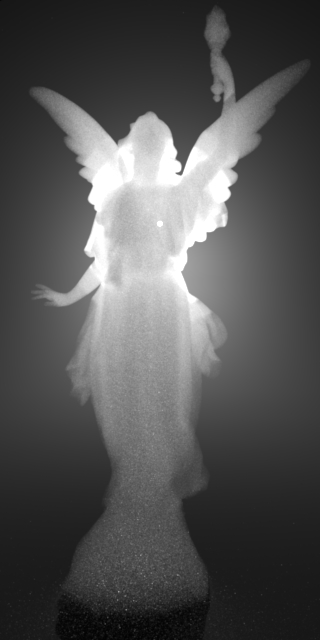
\includegraphics[width=\resLen]{waveoptics/lucy/pos_unc.jpg} &
        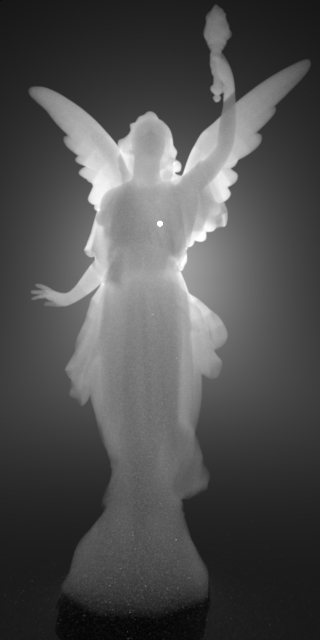
\includegraphics[width=\resLen]{waveoptics/lucy/pos_pos.jpg} 
        \\
        \textbf{(a1)} unc. clusters & \textbf{(a2)} neg. clusters & \textbf{(b1)} unc. clusters & \textbf{(b2)} pos. clusters
    \end{tabular}
    \caption[Correlated particles]{\label{fig:waveoptics:correlated}
        \textbf{Correlated particles:} By correlating particle positions in negatively (a) or positively (b), our method can produce bulk scattering parameters for correlated media.
        In this example, we use $\lambda = 400\text{nm}$, particle radius $a_i = 500\text{nm}$, and per-cluster particle count $\Ncls = 100$.
        Additionally, we can further correlate particle clusters themselves, a variety of appearances can be achieved (\textbf{a1--b2}).
        (The bright dot in \textbf{(b1)} and \textbf{(b2)} emerges from unscattered light from the area source.)
    }
\end{figure}

